\documentclass[12pt]{article}

% This first part of the file is called the PREAMBLE. It includes
% customizations and command definitions. The preamble is everything
% between \documentclass and \begin{document}.

\usepackage[margin=1in]{geometry}  % set the margins to 1in on all sides
\usepackage{graphicx}              % to include figures
\usepackage{amsmath}               % great math stuff
\usepackage{amsfonts}              % for blackboard bold, etc
\usepackage{amsthm}                % better theorem environments


% various theorems, numbered by section

\newtheorem{thm}{Theorem}[section]
\newtheorem{lem}[thm]{Lemma}
\newtheorem{prop}[thm]{Proposition}
\newtheorem{cor}[thm]{Corollary}
\newtheorem{conj}[thm]{Conjecture}

\DeclareMathOperator{\id}{id}

\newcommand{\bd}[1]{\mathbf{#1}}  % for bolding symbols
\newcommand{\RR}{\mathbb{R}}      % for Real numbers
\newcommand{\ZZ}{\mathbb{Z}}      % for Integers
\newcommand{\col}[1]{\left[\begin{matrix} #1 \end{matrix} \right]}
\newcommand{\comb}[2]{\binom{#1^2 + #2^2}{#1+#2}}


\begin{document}


\nocite{*}

\title{A Sample Mathematics Paper}

\author{Edward R. Scheinerman\thanks{Grant support listed here.} \\ 
Department of Applied Mathematics and Statistics \\
The Johns Hopkins University \\
Baltimore, Maryland 21218 USA}

\maketitle

\begin{abstract}
  This is a sample \LaTeX\ paper; its purpose is to show the basics of
  setting up a paper and important features of \LaTeX. It can also be
  used for assignments or other short notes.
\end{abstract}


\section{Introduction}

This is a simple \LaTeX\ document designed to illustrate the basics of
typesetting a paper. The ideas shown here can be adapted for
a more informal document, such as a homework assignment. 

This document is created from various source files, the most important
of which is named \verb|paper.tex|. By reading \verb|paper.tex| along
side the typeset output, the diligent reader should be able to deduce
how various parts of \LaTeX\ work. Indeed, you cannot understand
everything that we did in this paper without looking at the source
file. For example, how did we type \LaTeX?

Remember that \LaTeX\ is a markup language and not a
what-you-see-is-what-you-get word processor. 

Good luck.

\section{Basic Stuff}
\label{sect:basics}


\subsection{Files and commands}

\LaTeX\ converts files you type into professional-looking typeset
documents. You type your \LaTeX\ document using a text editor (such as
Emacs on a Unix computer or in an integrated editor in a \TeX\
system). This file's name should end ``\verb|.tex|''. The file that
produced this document is named \verb|paper.tex|.


To convert a source file, such as \verb|paper.tex|, into a finished
product (in \verb|PDF| format) one gives a command\footnote{For papers
  with cross references it may be necessary to run `pdflatex` more
  than once.}
such as this:
\begin{verbatim}
pdflatex paper
\end{verbatim}
An integrated \LaTeX\ system will have a menu item named ``Typeset''
(or something simimlar) to process your file.


\subsection{Skeleton of a \LaTeX\ document} 

The first line of a typical \LaTeX\ document is this:
\begin{verbatim}
\documentclass[12pt]{article}
\end{verbatim}
(The optional \verb|[12pt]| sets the overall point size for the main
text of your document to 12~points. You may use \verb|[11pt]| for
11~point text or omit this for 10~point.)

The lines immediately following \verb|\documentclass| are known as the
\emph{preamble} of your document. This is where you define your own
commands, load optional packages, etc. In the simple
\verb|hello-world.tex| file, there are no lines in the preamble
section. For this document, there are several.

The main text of the document is enclosed between lines that say
\verb|\begin{document}| and \verb|\end{document}|. This is where you
type the words you want to appear on your paper. (Look for those lines
now in the file \verb|paper.tex|.)


\subsection{Typing and fonts}
\label{subsect:typing}


To type ordinary text, simply type what you want. To start a new
paragraph, simply skip a line.


Certain characters have special meanings. The two most important are
the backslash (\verb|\|) and the dollar sign (\verb|$|). Most \LaTeX\
commands are preceded by a backslash. All mathematical symbols should
be enclosed by dollar signs. If you need a dollar sign in ordinary
text, you can type \verb|\$| to produce, say, ``Dan Naiman owes me
\$5.'' I can't think of any occasion where you need a backslash in
ordinary text. (You cannot produce a backslash in ordinary text by
typing \verb|\\|.)

Use the correct quotation marks. To enclose words in double quotes,
begin with two back tick characters\footnote{On many keyboards, you
will find the back tick character in the top row to the extreme left.}
\verb|``| and end with two apostrophes \verb|''|. Do not use the
double quote key \verb|"|. To enclose words in single quotes, begin
with a single back tick character and end with a single apostrophe.

Typically, you should not need to change the size of the text you are
typing. Use the logical structures of \LaTeX\ and let the computer
pick the appropriate size.\footnote{For example, text in a footnote is
automatically typeset smaller than text in the main body of the
document.}  The overall point size of the document is indicated at the
beginning of the file as an optional argument to the
\verb|\documentclass| command.

Likewise with font style. In general, you do not need to pick the
font. Variable names in mathematics mode are automatically typeset in
italics as in $x+1$. Similiarly, the font style in section heads, theorems,
etc., are automatically produced for you. For example:

\begin{thm} \label{thm:pyth}
  Suppose the lengths of the legs of a right triangle are $a$ and $b$,
  and the length of the hypotenuse is $c$. Then $a^2+b^2=c^2$.\qed
\end{thm}

However, there are times you may wish to use italics to show
emphasis. To do this enclose your text in \verb|\emph{...}| as in: I
am \emph{still} waiting for him to pay me back. 

\emph{Never use mathematics mode to typeset ordinary text in
  italics.} If you do, the result will look $awful$. 

To typeset in boldface enclose your text in \verb|\textbf{...}| and to
typeset in sans serif enclose in \verb|\textsf{...}|. However, you
probably will not need to use these in ordinary text. (Later we talk
about math typeset in bold, e.g., for vectors.) 

To typeset in \textsc{Caps and Small Caps} use \verb|\textsc{...}|. To
typeset in \texttt{typewriter font} use \verb|\texttt{...}|. However,
to show something that looks like computer code, you probably want to
use one of the verbatim methods; look inside this document to figure
out how we did it. The starred version of the verbatim environment 
shows spaces with a \verb*|funny little symbol|. 

The system of fonts used by \LaTeX\ is known as the Computer Modern
family. If you prefer Times Roman, include these commands in the
preamble of your file:
\begin{verbatim}
\usepackage{times}
\usepackage{mathptm}
\end{verbatim}

\subsection{Accents}

Don't be na\"{\i}ve, ordering \'a la carte is expensive. Don't use \"o
when you write Erd\H{o}s. Be honest; don't put up a fa\c{c}ade. Use
H\^opital's rule.


\subsection{Lists}

For numbered lists use the \verb|enumerate| enviroment and for
bulleted lists use the \verb|itemize| environment as in these
examples.

This is a numbered list.
\begin{enumerate}
\item If you loan money to faculty members, be sure to get an I.O.U.
\item To be sure that students show up for events, serve food.
\end{enumerate}

This is a bulleted list.
\begin{itemize}
\item \LaTeX\ does an excellent job of typesetting mathematics
  papers. 
\item \LaTeX\ can easily produce beautiful results that are 99\%
  perfect.
\item You can drive yourself crazy on that last 1\%. Don't bother.
\end{itemize}

You can nest these types of lists inside each other. 

\section{Mathematics}

\subsection{Basic math}

Whenever you typeset mathematical notation, it needs to be inside a
mathematics environment. The simplest way to do this is to enclose the
notation between single dollar signs \verb|$|. For example: If $a$ is
an integer, then $2a+1$ is odd. 

Superscripts and subscripts are created using the characters \verb|^|
and \verb|_|, respectively: $x^2+y^2=1$ and $a_n=0$. It is fine to
have both on a single letter: $x_0^2$.

If the superscript [or subscript] is more than a single character,
enclose the superscript in curly braces: $e^{-x}$. 

Greek letters are typed using commands such as \verb|\gamma|
($\gamma)$ and \verb|\Gamma| ($\Gamma$).

Named mathematics operators are usually typeset in roman. Most of the
standards are already available. Some examples: $\det A$, $\cos\pi$,
and $\log(1-x)$. If \LaTeX\ doesn't already have the operator you
like, you can create your own\footnote{This requires the
\texttt{amsmath} package; see \cite{amsldoc}.} using
the \verb|DeclareMathOperator| command. For example, to make
\verb|\id| the identity operator:
\begin{verbatim}
\DeclareMathOperator{\id}{id}
\end{verbatim}
Now we can type \verb|$\id(x)$| to produce $\id(x)$. The
\verb|\DeclareMathOperator| command must go in the preamble (before
\verb|\begin{document}|). 


\subsection{Displayed equations}

When an equation becomes too large to run in-line, you display it on a
line by itself by enclosing it in double dollar signs \verb|$$|. 
$$
f(x) = 5x^{10}-9x^9 + 77x^8 + 12x^7 + 4x^6 - 8x^5 + 7x^4 + x^3 -2x^2 +
3x + 11.
$$

If you want a numbered equation, enclose it in \verb|\begin{equation}|
and \verb|\end{equation}|.
\begin{equation} \label{eq:polynomial}
g(x) = x^{10}+x^9 - x^3 -x -1.
\end{equation}
The numbering is automatically provided by \LaTeX.

If you want to number an equation with your own number (don't!) or
symbol (maybe), you can do this:
$$
h(x) = f(x)+g(x). \eqno{(*)}
$$

The \verb|\begin{align*}...\end{align*}| environment is superb for
lining up equations. (Omit the \verb|*| for numbered equations.)
\begin{align*}
  (x-y)^2 
  &= (x-y)(x-y)\\
  &= x^2 -yx - xy + y^2 \\
  &= x^2 -2xy +y^2.
\end{align*}

\begin{align*}
3x-y&=0 & 2a+b &= 4 \\
x+y &=1 & a-3b &=10
\end{align*}

To insert ordinary text inside of mathematics mode, use \verb|\text|:
$$
f(x) = \frac{x}{x-1} \text{ for $x\not=1$}. 
$$
This is the $3^{\text{rd}}$ time I've asked for my money back.

The \verb|\begin{cases}...\end{cases}| environment is perfect for
defining functions piecewise:
$$
|x| = 
\begin{cases}
x & \text{when $x \ge 0$ and} \\
-x & \text{otherwise.}
\end{cases}
$$

\subsection{Relations and operations}

\begin{itemize}

\item Equality-like: $x=2$, $x \not= 3$, $x \cong y$, $x \propto y$, $y\sim
z$, $N \approx M$, $y \asymp z$, $P \equiv Q$.

\item Order: $x < y$, $y \le z$, $z \ge 0$, $x \preceq y$, $y\succ z$,
  $A \subseteq B$, $B \supset Z$.

\item Arrows: $x \to y$, $y\gets x$, $A \Rightarrow B$, $A \iff B$, 
$x \mapsto f(x)$, $A \Longleftarrow B$. 

\item Set stuff: $x \in A$, $b \notin C$, $A \ni x$. Use
  \verb|\notin| rather than \verb|\not\in|. 
  $A \cup B$, $X \cap Y$, $A \setminus B = \emptyset$. 

\item Arithmetic: $3+4$, $5-6$, $7\cdot 8 = 7\times8$,
  $3\div6=\frac{1}{2}$, $f\circ g$, $A \oplus B$, 
  $v \otimes w$. 

\item Mod: As a binary operation, use \verb|\bmod|: $x \bmod N$. As a
  relation use \verb|\mod|, \verb|\pmod|, or \verb|\pod|: 
  \begin{align*}
    x &\cong y \mod 10 \\
    x &\cong y \pmod{10} \\
    x &\cong y \pod{10}
  \end{align*}

\item Calculus: $\partial F/\partial x$, $\nabla g$.
  

\end{itemize}


\subsection{Use the right dots}

Do not type three periods; instead use \verb|\cdots| between
operations and \verb|\ldots| in lists:
$x_1 + x_2 + \cdots + x_n$ and $(x_1,x_2,\ldots,x_n)$. 



\subsection{Built up structures}

\begin{itemize}

\item Fractions: $\frac{1}{2}$, $\frac{x-1}{x-2}$.

\item Binomial coefficients: $\binom{n}{2}$.

\item Sums and products. Do \emph{not} use \verb|\Sigma| and \verb|\Pi|. 
$$
\sum_{k=0}^\infty \frac{x^k}{k!} \not= \prod_{j=1}^{10} \frac{j}{j+1}.
$$
$$
\bigcup_{k=0}^\infty A_k
\qquad
\bigoplus_{j=1}^\infty V_j
$$

\item Integrals:
  $$
  \int_0^1  x^2 \, dx
  $$
  The extra bit of space before the $dx$ term is created with the
  \verb|\,| command.

\item Limits:
  $$
  \lim_{h\to0} \frac{\sin(x+h) - \sin(x)}{h} = \cos x .
  $$
  Also $\limsup_{n\to\infty} a_n$. 
  

\item Radicals: $\sqrt{3}$, $\sqrt[3]{12}$, $\sqrt{1+\sqrt{2}}$.

\item Matrices:
  $$
  A = \left[\begin{matrix} 3 & 4 & 0 \\ 2 & -1 & \pi \end{matrix}\right] .
  $$ 
  In line: 
  $A = \left[\begin{smallmatrix}1 & 0 \\ 0 &
  1\end{smallmatrix}\right]$.
  A big matrix:
  $$
  D = \left[ 
    \begin{matrix}
      \lambda_1 & 0 & 0 & \cdots & 0 \\
      0 & \lambda_2 & 0 & \cdots & 0 \\
      0 & 0 & \lambda_3 & \cdots & 0 \\
      \vdots & \vdots & \vdots & \ddots & \vdots \\
      0 & 0 & 0 & \cdots & \lambda_n
    \end{matrix}
    \right].
  $$
  
\end{itemize}

\subsection{Delimiters}

\begin{itemize}

\item Parentheses and square brackets are easy: 
  $(x-y)(x+y)$, $[3-x]$.

\item For curly braces use \verb|\{| and \verb|\}|:
  $\{x : 3x-1 \in A\}$. 

\item Absolute value: $|x-y|$, $\|\vec{x} - \vec{y}\|$. 

\item Floor and ceiling: $\lfloor \pi \rfloor = \lceil e \rceil$. 


\item To make delimiters grow so they are properly sized to contain
their arguments, use \verb|\left| and \verb|\right|:
$$
\left[ \sum_{n=0}^\infty a_n x^n \right]^2 =
\exp \left\{ - \frac{x^2}{2} \right\}
$$

Occasionally, it is useful to coerce a larger sized delimiters than 
\verb|\left|/\verb|\right| produce. Look at the two sides of this
equation:
$$ 
\left((x_1+1)(x_2-1)\right)
=
\bigl((x_1+1)(x_2-1)\bigl).
$$
I think the right is better. Use \verb|\bigl|, \verb|\Bigl|,
\verb|\biggl|, and the matching \verb|\bigr|, etc. 

\item Underbraces:
  $$ 
  \underbrace{1+1+\cdots+1}_{\text{$n$ times}} = n .
  $$


\end{itemize}

\subsection{Styled and decorated letters}

\begin{itemize}

\item Primes: $a'$, $b''$.

\item Hats: $\bar a$, $\hat a$, $\vec a$, $\widehat{a_j}$. 

\item Vectors are often set in bold: $\mathbf{x}$. Don't use
  \verb|\textbf| in mathematics mode and don't use \verb|\mathbf| in
  text mode.

\item Calligraphic letters (for sets of sets): $\mathcal{A}$.

\item Blackboard bold for number systems: $\mathbb{C}$.

\end{itemize}



\subsection{Defining your own commands}

You can (and should) define your own commands (also called
macros). For example, if you refer to the positive orthant
$\mathbb{R}^n_+$ frequently, put the following line in your preamble:
\begin{verbatim}
\newcommand{\rnp}{\mathbb{R}^n_+}
\end{verbatim}
Then, you can just type \verb|$\rnp$| instead of
\verb|$\mathbb{R}^n_+$|. Also, if later you decide that you prefer
$\mathbf{R}$ instead of $\mathbb{R}$, you only have to change the
definition of \verb|\rnp|.

It is possible to define commands that take arguments. For example,
suppose your paper uses column vectors frequently. We define a new
command named \verb|\col| like this:
\begin{verbatim}
\newcommand{\col}[1]{\left[\begin{matrix} #1 \end{matrix} \right]}
\end{verbatim}
The \verb|[1]| means that \verb|\col| takes one argument. The
\verb|#1| shows where that one argument goes. Now we can type
$$
\col{1\\2\\3} + \col{-1\\3\\-2} = \col{0\\5\\1} 
$$
easily.

Here's another example. Suppose the expression $\comb{a}{b}$ appears
often (but with different values for $a$ and $b$). Let's call the
combinatorial oddity \verb|\comb| and define it like this:
\begin{verbatim}
\newcommand{\comb}[2]{\binom{#1^2 + #2^2}{#1+#2}}
\end{verbatim}
and use it like this: \verb|$\comb{a}{b}$|. 

\section{Theorem/Proof}

In the preamble of this document, find the following lines:
\begin{verbatim}
\newtheorem{thm}{Theorem}[section]
\newtheorem{lem}[thm]{Lemma}
\newtheorem{prop}[thm]{Proposition}
\newtheorem{cor}[thm]{Corollary}
\newtheorem{conj}[thm]{Conjecture}
\end{verbatim}

The first line defines a \verb|\begin{thm}...\end{thm}|
environment. This will produce a theorem named ``Theorem'' and the
numbering style will be based on the section (e.g., Theorem~2.1); omit
the \verb|[section]| and the numbering will be absolute (e.g.,
Theorem~1).

The second line defines a \verb|\begin{lem}...\end{lem}|
environment to produce theorems marked ``Lemma''. The \verb|[thm]|
means that this environment shares the same numbering as \verb|thm|. 

So we get this:

\begin{thm} 
  A subset of the real line is compact if and only if it is closed and
  bounded. 
\end{thm}

\begin{lem}
  In any graph, the sum of the degrees of the vertices is twice the
  number of edges.
\end{lem}

\begin{conj}
  All perfect numbers are even.
\end{conj}


Theorems with names can have those names inserted like this:

\begin{thm}[Fundamental Theorem of Algebra]
  Let $p$ be a polynomial with complex coefficients. Then there exists
  $z \in \mathbb{C}$ such that $p(z)=0$.
\end{thm}

Enclose your proof in a \verb|\begin{proof}...\end{proof}|
environment.\footnote{You need the \texttt{amsthm} package for this;
  see \cite{amsldoc} and \cite{amsthdoc}.}

\begin{proof}
Let $X$ be the set of all positive integers that are not
interesting. Suppose, for the sake of contradiction, that
$X\not=\emptyset$. By the well-ordering principle, $X$ contains a
least element $a$. Note that $a$ is the first noninteresting number,
but that's interesting! $\Rightarrow\Leftarrow$. Therefore,
$X=\emptyset$ and so all positive integers are interesting.
\end{proof}

Note that the end-of-proof symbol is automatically included. To show
that a proof of a theorem is omitted, you can add an end-of-proof
symbol yourself using the \verb|\qed| command.

\begin{prop}
  Let $x$ be an integer. Then $x$ is even if and only if $x+1$ is
  odd.\qed 
\end{prop}


\section{Cross References}
\label{sect:cross-ref}

\subsection{Labels for numbered entities}

Numbered \LaTeX\ structures can be given a label and we can use that
label to refer to that structure. For example, this section is labeled
using the command \verb|\label{sect:cross-ref}|. That enables me to
type \verb|Section~\ref{sect:cross-ref}| to produce
``Section~\ref{sect:cross-ref}''. The tilde \verb|~| is called a
``tie'' character. It produces a space but \LaTeX\ won't break the
line at that point.

It is much better to use labels and references than to type in the
section (or theorem or subsection or figure or equation) number
yourself. If you change the document, the labels will change
automatically. 

You can use \verb|\pageref| to give the page number on which the label
can be found. For example, Theorem~\ref{thm:pyth} is on
page~\pageref{thm:pyth}. Don't use this for journal submissions.

You can use \verb|\eqref| to refer to equations; this command inserts
the parentheses for you: The polynomial $g$ is defined in
Equation~\eqref{eq:polynomial}.


\subsection{Citations}

Most papers contain references. The best way to deal with references
in \LaTeX\ is as follows:
\begin{itemize}
\item Have a separate bibtex file; the bibtex file for this paper is
  named \verb|paper.bib|. The bibtex file contains all the information
  about the references but no formatting information. Examine the
  \verb|paper.bib| file that accompanies this document.

\item At the end of the paper, please find these lines
\begin{verbatim}
\bibliographystyle{plain}
\bibliography{paper}
\end{verbatim}
The first specifies the bibliography style. (We chose ``plain'' but there
are others available.) The second builds the actual References section
of the paper. 

\item Each entry in the bibtex file has a key name. For example, the
  key for Knuth's \emph{\TeX book} is \verb|knuth84|. To include a
  reference in the paper to this book, we type \verb|\cite{knuth84}|
  to give this: \cite{knuth84}. 

\item Normally, only references that are cited with a \verb|\cite|
  command appear in the paper's bibliography. However, to coerce
  \LaTeX\ to include \emph{all} references in the bibtex file into
  your bibliography, include the command \verb|\nocite{*}| just after
  the \verb|\begin{document}| command.

\end{itemize}

To process the files \verb|paper.tex| and \verb|paper.bib|, run these
commands on your computer:
\begin{verbatim}
pdflatex paper
bibtex paper
pdflatex paper
pdflatex paper
\end{verbatim}




\section{Figures}
\label{sect:figures}

To incorporate a diagram into \LaTeX\ you first prepare that diagram
in a separate drawing program such as \verb|xfig|,
\emph{Mathematica}, or \textsc{Matlab}. Save your illustration in
\verb|pdf| format; let's say the file is called \verb|doodle.pdf|. 
We now want it to appear in our paper (as Figure~\ref{fig:doodle}).
\begin{figure}[ht]
\begin{center}
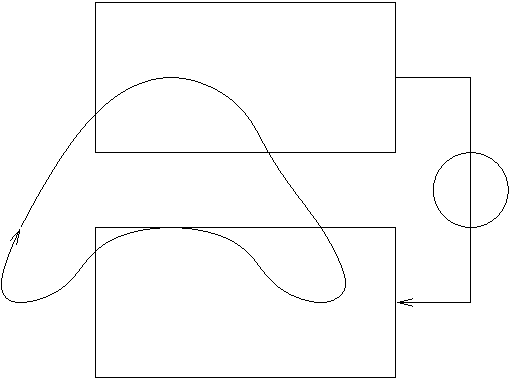
\includegraphics[scale=0.5]{doodle}
\end{center}
\caption{A doodle created with the Xfig program.}
\label{fig:doodle}
\end{figure}
The \LaTeX\ code that make the figure appear is this:
\begin{verbatim}
\begin{figure}[ht]
\begin{center}
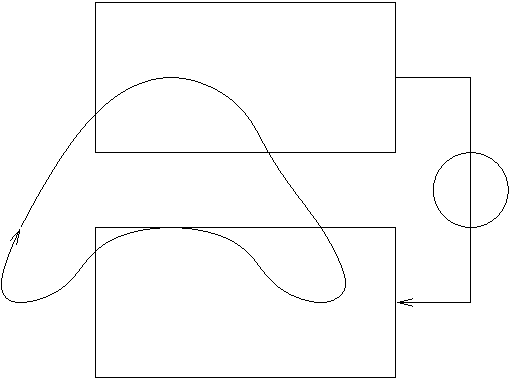
\includegraphics[scale=0.5]{doodle}
\end{center}
\caption{A doodle created with the Xfig program.}
\label{fig:doodle}
\end{figure}
\end{verbatim}

The optional \verb|[ht]| means that the figure may appear either
``Here'' or else at the ``Top'' of the next page (if it doesn't fit
here). \LaTeX\ takes these as suggestions and may decide to put your
figure somewhere else if the figure is too big. 

The optional \verb|[scale=0.5]| shrinks the image by 50\%.  Try
\verb|[width=\textwidth]| to make the figure exactly as wide as your
text.  Or \verb|[width=0.75\textwidth]| makes it $\frac34$ of the
width of your text.

\section{Tables}

Here are some simple examples of tables. Examine the source file to
see how they are created.

\begin{center}
\begin{tabular}{l|c|r}
Left flush & Centered & Right Flush \\
\hline
Row 1 & Middle of row one & right side of row I \\
A second row & row \#2 & R2
\end{tabular}
\end{center}

\begin{center}
\begin{tabular}{|c||c|c|c|c|}
\hline
$x$ & 1 & 2 & 3 & 4 \\
\hline
$x^2$ & 1 & 4 & 9 & 16 \\
\hline
\end{tabular}
\end{center}

\begin{center}
\begin{tabular}{|l|l|}
\hline
\textbf{Term} & \textbf{Definition} \\
\hline
\hline
symmetric & a matrix equal to its own transpose \\
\hline
singular & a matrix that is noninvertible \\
\hline
doubly stochastic & 
a nonnegative matrix whose rows and columns sum to one
\\
\hline
\end{tabular}
\end{center}

\section{Futher Reading}

The canonical introduction to \LaTeX\ is \cite{lamport}. I am
particularly fond of the American Mathematics Society's add-ons to
\LaTeX\ and these are documented in \cite{amsldoc} and
\cite{amsthdoc}.

More advanced information can be found in \cite{latex-companion}, 
\cite{math-into-latex}, and \cite{kopka03}. See also
\cite{latex-graphics} for more on graphics and \LaTeX. 

The \LaTeX\ system is built on top of Donald Knuth's \TeX; this is
documented in \cite{knuth84}, but you probably won't need to read
this. 

Searching for help on \LaTeX\ and bibtex on the web is often fruitful.

Please note that some of the entries in the bibliography (look inside
\verb|paper.bib|) are phony; they are included only to illustrate
different types of bibliographic entries. 


\bibliographystyle{plain}

\bibliography{paper}


\end{document}
